% author Truong Nhan Nguyen
% created in 11/1/2022

\documentclass[tikz, border=10pt]{standalone}

\usepackage{tikz}
\usepackage{amsmath, amssymb, amsfonts, mathtools}

\begin{document}
    \bfseries\sffamily\footnotesize
    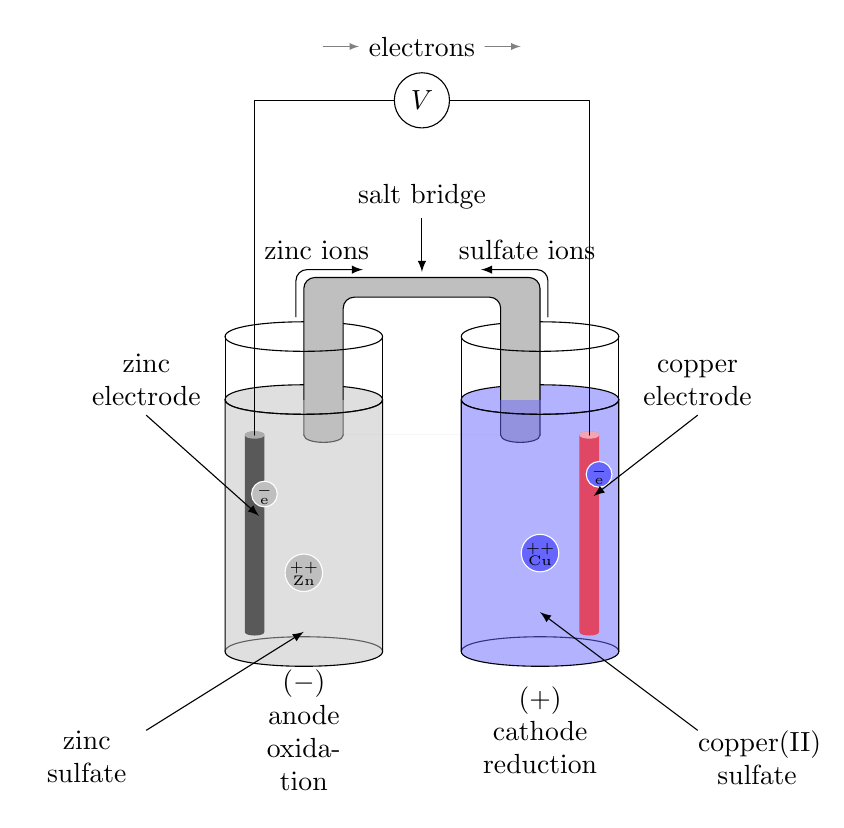
\begin{tikzpicture}[line cap=round, line join=round]
        % draw back side of first vessel (left vessel)
        \draw (0, 4) to[controls=+(90:0.25) and +(90:0.25)] (2, 4);
        \path[draw, fill=black!25, fill opacity=0.5] (0, 3.2) to [controls=+(90:0.25) and +(90:0.25)](2, 3.2);
        \draw (0, 0) to[controls=+(90:0.25) and +(90:0.25)] (2, 0);
        % draw back side of second vessel (right vessel)
        \draw (3, 4) to[controls=+(90:0.25) and +(90:0.25)] (5, 4);
        \path[draw, fill=blue!60, fill opacity=0.5] (3, 3.2) to [controls=+(90:0.25) and +(90:0.25)](5, 3.2);
        \draw (3, 0) to[controls=+(90:0.25) and +(90:0.25)] (5, 0);
        % draw salt bridge
        \path[draw, rounded corners, fill=black!25] (1, 2.75) -- (1, 4.75) -- (4, 4.75) -- (4, 2.75) (3.5, 2.75) -- (3.5, 4.5) -- (1.5, 4.5) -- (1.5, 2.75);
        \path[draw, fill=black!25] (1, 2.75) to[controls=+(-90:0.125) and +(-90:0.125)] (1.5, 2.75);
        \path[draw, fill=black!25] (4, 2.75) to[controls=+(-90:0.125) and +(-90:0.125)] (3.5, 2.75);
        % draw front side of first vessel
        \draw (0, 4) to[controls=+(-90:0.25) and +(-90:0.25)] (2, 4);
        \path[draw, fill=black!25, fill opacity=0.5] (0, 3.2) to [controls=+(-90:0.25) and +(-90:0.25)](2, 3.2);
        \draw (0, 4) -- (0, 3.2) (2, 4) -- (2, 3.2);
        \path[draw, fill=black!25, fill opacity=0.5] (0, 3.2) -- (0, 0) ..controls +(-90:0.25) and +(-90:0.25).. (2, 0) -- (2, 3.2) ..controls +(-90:0.25) and +(-90:0.25).. (0, 3.2);
        % draw front size of second vessel
        \draw (3, 4) to[controls=+(-90:0.25) and +(-90:0.25)] (5, 4);
        \draw  (3, 4) -- (3, 3.2) (5, 4) -- (5, 3.2);
        \path[draw, fill=blue!60, fill opacity=0.5] (3, 3.2) to [controls=+(-90:0.25) and +(-90:0.25)](5, 3.2);
        \path[draw, fill=blue!60, fill opacity=0.5] (3, 3.2) -- (3, 0) ..controls +(-90:0.25) and +(-90:0.25).. (5, 0) -- (5, 3.2) ..controls +(-90:0.25) and +(-90:0.25).. (3, 3.2);
        % draw left electrode
        \fill[black, fill opacity=0.6] (0.25, 0.25) ..controls +(-90:0.0625) and +(-90:0.0625).. (0.5, 0.25) -- (0.5, 2.75) ..controls +(90:0.0625) and +(90:0.0625).. (0.25, 2.75);
        \fill[black!10, fill opacity=0.6] (0.5, 2.75) .. controls +(-90:0.0625) and +(-90:0.0625).. (0.25, 2.75) .. controls +(90:0.0625) and +(90:0.0625).. (0.5, 2.75);
        % draw right electrode
        \fill[red, fill opacity=0.6] (4.5, 0.25) ..controls +(-90:0.0625) and +(-90:0.0625).. (4.75, 0.25) -- (4.75, 2.75) ..controls +(90:0.0625) and +(90:0.0625).. (4.5, 2.75);
        \fill[red!10, fill opacity=0.6] (4.75, 2.75) .. controls +(-90:0.0625) and +(-90:0.0625).. (4.5, 2.75) .. controls +(90:0.0625) and +(90:0.0625).. (4.75, 2.75);
        % draw voltage meter
        \node [draw, circle] (voltage) at (2.5, 7) {$V$};
        \draw (0.375, 2.75) |- (voltage) -| (4.625, 2.75);
        % draw zincs ion flow
        \draw[-latex, rounded corners] (0.9, 4.25) |- node[right=7.5pt, above] {zinc ions} (1.75, 4.85);
        % draw sulfate ions flow
        \draw[-latex, rounded corners] (4.1, 4.25) |- node[left=7.5pt, above] {sulfate ions} (3.25, 4.85);     
        % draw salt bridge label
        \draw[-latex, shorten >=2pt] (2.5, 5.5) node[anchor=south] {salt bridge} -- (2.5, 4.75);
        % draw electrons flow
        \node[
            yshift=-9pt, pin={[pin edge={latex-}]180:$ $}, pin={[pin edge={-latex}]0:$ $}
        ] (electrons) [above of=voltage] {electrons};
        % draw anode and cathode
        \node[text width=1.2cm, text centered] at (1, -1) {$(-)$ anode oxidation};
        \node[text width=1.5cm, text centered] at (4, -1) {$(+)$ cathode reduction};
        % draw ions
        \node[draw=white, circle, fill=black!25, inner sep=0pt] at (1, 1) {\tiny$\overset{++}{\mathrm{Zn}}$};
        \node[draw=white, circle, fill=blue!60, inner sep=0pt] at (4, 1.25) {\tiny$\overset{++}{\mathrm{Cu}}$};
        \node[draw=white, circle, fill=black!25, inner sep=0pt] (e1) at (0.5, 2) {\tiny$\overset{-}{\mathrm{e}}$};
        \node[draw=white, circle, fill=blue!60, inner sep=0pt] (e2) at (4.75, 2.25) {\tiny$\overset{-}{\mathrm{e}}$};
        % draw texts
        \draw[-latex] (-1, 3) node[text width=1.5cm, text centered, anchor=south] {zinc electrode} -- ([yshift=-3pt, xshift=-2pt]e1.south);
        \draw[-latex] (-1, -1) node[text width=1.5cm, text centered, anchor=north east, inner sep=0pt] {zinc sulfate} -- (1, 0.25);
        \draw[-latex] (6, 3) node[text width=1.5cm, text centered, anchor=south] {copper electrode} -- ([yshift=-3pt, xshift=-2pt]e2.south);
        \draw[-latex] (6, -1) node[text width=1.5cm, text centered, anchor=north west, inner sep=0pt] {copper(II) sulfate} -- (4, 0.5); 
    \end{tikzpicture}
\end{document}